%
%  version 1, 2016-12-05
%
\documentclass[twocolumn,twoside]{svmultivs_br} %please do not change this line
\usepackage{graphicx}
%
% The contents of \title* are printed on the first page.
% The contents of \subtitle are printed below the title on the
% first page.  This keyword is optional.
% The contents of \titlerunning are printed on the other pages.
% This should be a short version of the title.
%
\title*{Norwegian Mapping Authority Analysis Center Biennial Report}
\subtitle{2015--2016}
\titlerunning{NMA AC 2015--2016 Report}
%
% Example:
% \title*{IVS Coordinating Center 2015---2016 Biennial Report}
% \titlerunning{IVS CC 2015---2016 Report}
%
% \subtitle may be used if there is not enough room in \title*.  
% Example:
% \title*{International VLBI Service Coordinating Center Biennial Report Submission}
% \subtitle{Work during 2015---2016}
% \titlerunning{IVS CC 2015---2016 Report}
%
\author{Ann-Silje Kirkvik}
\authorrunning{Kirkvik} % see comments below
\authoremails{ann-silje.kirkvik@kartverket.no}
\institute{Norwegian Mapping Authority (NMA)}
%
% \author and \institute keywords:
%
% Each number in \author refers to an institution with which the author is associated.
% The numbers should correspond to numbered institutions in the \institute keyword.
% If all authors are associated with only one institution (the same institution),
% then the numbers should be omitted from \author and \institute.
% If an author is associated with two or more institutions, multiple numbers may be
% used.
%
% The \institute key word must be a single line.
% Please separate institutions using \\ between each institution.
%
% \authorrunning keyword:
%
% For one author, please use \authorrunning{last_name_of_author},
% e.g., \authorrunning{Behrend}
% For two authors, please use \authorrunning{last_name_of_first_author and last_name_of_second_author}
% e.g., \authorrunning{Behrend and Baver}
% For three or more authors, please use \authorrunning{last_name_of_first_author et al.}
% e.g., \authorrunning{Behrend et al.}
%
% Examples
%
% \author{Dirk Behrend}
% \authorrunning{Behrend}
% \author_emails{dirk.behrend-1@nasa.gov}
% \institute{NVI, Inc.}
%
% \author{Karen Baver, Dirk Behrend}
% \authorrunning{Baver and Behrend}
% \author_emails{karen.d.baver@nasa.gov,dirk.behrend-1@nasa.gov}
% \institute{NVI, Inc.}
%
% \author{John Gipson~$^1$, David Eriksson~$^{1,2}$, Chopo Ma~$^3$}
% \authorrunning{Gipson et al.}
% \institute{1. NVI, Inc. \\ 2. Chalmers University of Technology \\ 3. Goddard Space Flight Center}
%
\component{NMA Analysis Center} 
%
% Examples:
%    Mets\"ahovi Network Station
%    NEOS Operation Center
%    Bonn Correlator
%    INAF Data Center
%    IAA Analysis Center
%    NICT Technology Development Center
%
% Exceptions are the coordinators, who should use
%    IVS Analysis Coordinator
% etc.
%    
% \ContactAuthorName, \ContactAuthorTelephone, and \ContactAuthorEmail 
% should be used to identify the preferred contact author.
%
\ContactAuthorName{Ann-Silje Kirkvik}
\ContactAuthorTelephone{+47 32118421}
\ContactAuthorEmail{ann-silje.kirkvik@kartverket.no}
%
\NumberofInstitutions{1}
\InstitutionPostAddress{1}{Postboks 600 Sentrum, 3507 Hønefoss}
\InstitutionCountry{1}{Norway}
\InstitutionWebPage{1}{http://www.kartverket.no}
%
% Example:
%
% \InstitutionPostAddress{1}{61 avenue de l'Observatoire, 75014 Paris}
% \InstitutionCountry{1}{France}
% \InstitutionWebPage{1}{http://www.obspm.fr}
%
\begin{document}  %please do not change this line
%
\maketitle       %please do not change this line
%
\abstract{In 2015 Norwegian Mapping Authority (NMA) decided to discontinue the development of GEOSAT. Instead the development of a new software called Where started. Where will continue with some of the ideas from GEOSAT, but with a more modern software architecture and technology platform. The VLBI version of Where was almost complete by the end of 2016. NMA participated in VASCC2015 using GEOSAT and intend to participate with Where in the next phase of the campaign. }
%
\section{General Information}
NMA has been an Associate Analysis Center within the IVS since 2010. The analysis center
is operated by the Geodetic Institute at NMA with main offices in H\o nefoss, Norway. NMA is a 
governmental agency and the IVS activities at NMA are completely funded by the Norwegian government.  

NMA was using the analysis software GEOSAT. GEOSAT was originally developed by Per Helge Andersen (retired) at the Norwegian 
Defense Research Establishment (NDRE). The GEOSAT source code was finally abandoned in favour of creating a new software
with an improved architecture and using a more modern technology platform. The new software is called Where. 

The new software should be able to process observations from VLBI, GNSS, SLR and DORIS and will become an important tool at
NMA for improving the global geodetic reference frame. Where is implemented in Python and utilizes several well known packages such as \texttt{numpy}, \texttt{scipy} and \texttt{matplotlib}. In addition, more specialized packages like \texttt{astropy}\footnote{http://www.astropy.org} and \texttt{jplephem}\footnote{https://pypi.python.org/pypi/jplephem} are also used. Where is a command line tool, but the the results can be inspected using the graphical tool called There that is developed alongside Where. 

\section{Staff}
The Geodetic Institute at NMA has approximately 50 employees. Some of the responsibilities include maintaining the national reference frame, geoid and height system. The Geodetic Institute also provides a network-RTK positioning service and operates the VLBI station at Ny-\AA lesund. The Where project team consists of six members. These members are briefly described in table \ref{tab:staff}.
\begin{table*}[htb!]
\caption{Where project team members}
\begin{center}
\begin{tabular}{p{0.3\textwidth}|p{0.35\textwidth}|p{0.35\textwidth}}
\hline
Name & Background & Tasks \\
\hline
Laila L\o vh\o iden & Oil industry and co-chairing the UN-GGIM working group & Project manager \\
Michael D\"ahnn & Dipl.-Ing. in geodesy from the Dresden University of Technology & GNSS implementation \\
Ingrid Fausk & Ph.D. in mathematics from the University of Oslo & SLR implementation \\
Geir Arne Hjelle & Ph.D. in mathematics from the Norwegian University of Science and Technology & Software architecture and assisting with all the techinques \\
Ann-Silje Kirkvik & M.Sc. in computer science from the Norwegian University of Science and Technology & VLBI implementation \\
Eirik Mysen & Ph.D. in astrophysics from the University of Oslo & Estimation techniques \\
\hline
\end{tabular}
\end{center}
\label{tab:staff}
\end{table*}


\section{Activities during the Past Year}
In 2015 NMA decided to participate in the VLBI Analysis Software Comparison Campaign (VASCC2015) organized by Ph.D student Grzegorz Klopotek at Chalmers University of Technology, Sweden. The goal of the campaign was to compare computed theoretical delays from different analysis software packages. NMA provided solutions using the GEOSAT software. 

This work was very time consuming, but turned out to be an extremely valuable experience. The need to modernize the software became exceedingly clear as GEOSAT was disassembled to be able to provide solutions for VASCC2015. GEOSAT provided consistent results compared with other software packages for geometrical, gravitational and tropospheric delay and delay due to axis offset and thermal deformation. Figure \ref{fig:c5++vsgeosat} shows that the difference between c5++ and GEOSAT is less than 1mm for all observations of that session. As mentioned in \cite{vascc2015}, the discrepancies between the software packages increased as high frequency EOP variations were included. The site displacement models still need to be compared. 

Development of Where started in the second half of 2015. The experience from VASCC2015 was very helpful when implementing the VLBI model in Where, but no source code from GEOSAT has been used in Where. Where uses external libraries and functions such as SOFA\footnote{http://www.iausofa.org/2015\_0209\_F/sofa/sofa\_pn.pdf} and the IERS Conventions 2010 software \footnote{http://maia.usno.navy.mil/conv2010/software.html}. When the VLBI model was implemented in Where the dataset from VASCC2015 was used to compare the theoretical delays with GEOSAT. The results are shown in figure \ref{fig:geosatvswhere} and they indicate that Where can calculate theoretical delays at the same level as the software packages that participated in VASCC2015. As with GEOSAT, the site displacement models and EOP variations still need more extensive testing. 

The Where project team visited Onsala Space Observatory in June 2016 where the group photo in figure \ref{fig:onsala} was taken. The goal of this meeting was to share experiences and explore future possibilities for collaborations. The space geodesy field is very small in Norway and being able to cooperate with similar groups in neighbouring countries would be very beneficial. The meeting went well and a new meeting is planned in February 2017 in Norway. This meeting also includes Toshimichi Otsubo, who is on a sabbatical at Onsala Space Observatory, which provides an excellent opportunity to learn about the SLR implementation in c5++.


\begin{figure}[htb!]
\centering
\includegraphics[width=\linewidth]{acnma01.pdf}
\caption{Comparison of theoretical delays between c5++ and GEOSAT for the session 15JUN22CC\_NH. Includes geometrical, gravitational, tropspheric delay and delay due to axis offset. High freqency EOP variations and station displacement models are not included. Figure provided by Grzegorz Klopotek.}
\label{fig:c5++vsgeosat}
\end{figure}

\begin{figure}[htb!]
\centering
\includegraphics[width=\linewidth]{acnma02.pdf}
\caption{Comparison of theoretical delays between GEOSAT and Where for the session 15JUN22CC\_NH. Includes geometrical, gravitational, tropspheric delay and delay due to axis offset. High freqency EOP variations and station displacement models are not included.}
\label{fig:geosatvswhere}
\end{figure}

\begin{figure*}[htb!]
\centering
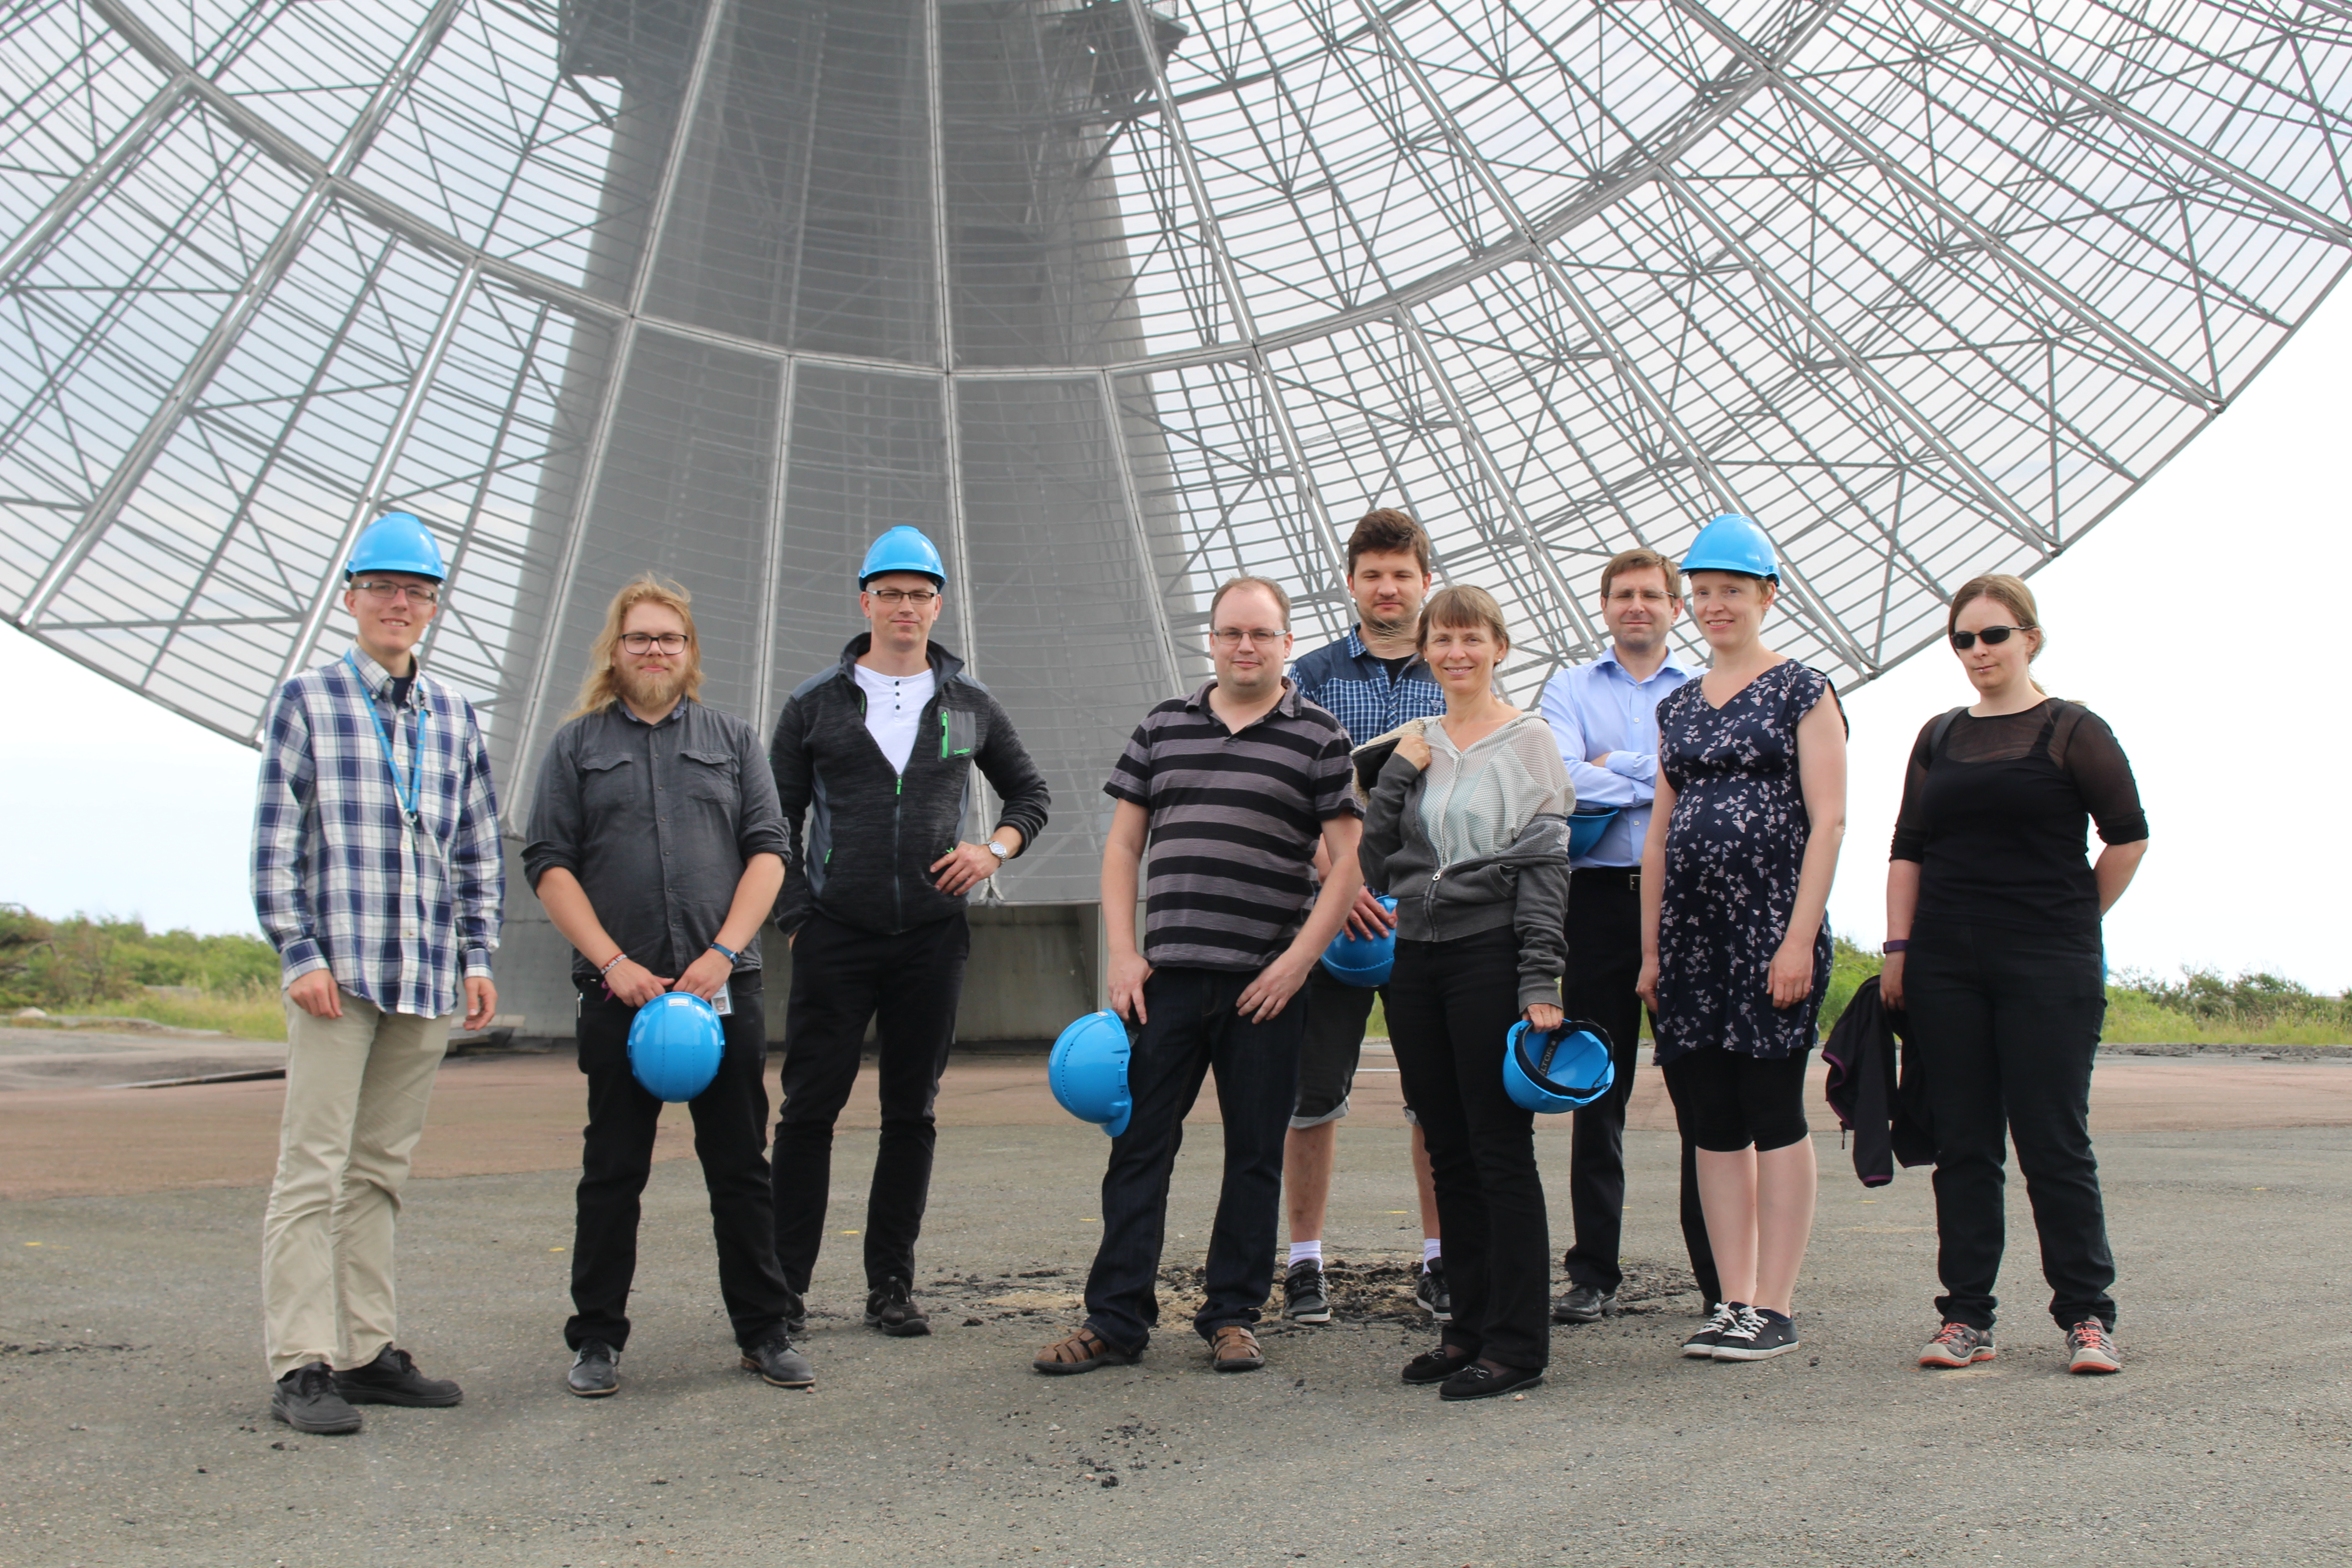
\includegraphics[width=\textwidth]{acnma03.JPG}
\caption{Visit at Onsala Space Observatory in June 2016. Back row from the left: Grzegorz Klopotek, Thomas Hobiger. Front row from the left: Joakim Strandberg, Niko Kareinen, Eirik Mysen, Geir Arne Hjelle, Laila L\o vh\o iden, Ingrid Fausk, Ann-Silje Kirkvik. Photo: Michael D\"{a}hnn.}
\label{fig:onsala}
\end{figure*}


%\FloatBarrier
\section{Current Status}
The VLBI implementation in Where is almost ready for a beta release. The software can read NGS files and applies a VLBI model consistent with conventions (\cite{iers2010}, \cite{deform}). Parameters are estimated using a Kalman filter (and smoother) where the nuisance parameters clocks and troposphere is modeled as continuous piecewise linear parameters. Using the results from \cite{neq}, it is possible to create unconstrained normal equations on SINEX format based on the Kalman filter solution. This requires that all target parameters are estimated as a constant for the whole session. 

The GNSS implementation is currently limited to GPS and the implementation of a Precise Point Positioning solution in Where, which is still under development. Development of SLR is halted due to maternity leave, but basic orbit determination is implemented. Development is expected to resume in the second half of 2017. Implementation of DORIS is completely on hold until the necessary resources becomes available.

\section{Future Plans}

The immediate main goal is to get a working version for VLBI analysis. The next step is to implement support for the new observation format vgosDb \cite{vgosdb}. It has also been announced that the VLBI Analysis Software Comparison Campaign will continue in 2017 and NMA intends to participate using Where. 

%
% Code to include a single column figure through \includegraphics.
% \begin{figure} and \end{figure} make this single column.
% If the figure is too wide, it will overwrite text in the other column.
% Figures should be centered through the latex \begin{center} and
% \end{center} commands.  
% Captions should be left-justified.  
% The class file will automatically perform the left-justification,
% if the caption is not included in the latex centering.
%
%\begin{figure}[htb!]         
%  \begin{center}
%
% Please specify the file extension as part of the figure
% file name. The formats of jpg, png and pdf can be used.
% Sample files names are: 
%       acgsfc01.jpg  
%       tdgsfc01.png and tdgsfc02.png
%       occore01.jpg, occore02.png, and occore03.pdf.
%
%  \includegraphics[width=.5\textwidth]{ivs-br-template01.jpg}
%%%%%  The caption should not be preceded by Figure 1.  
%%%%%  Please just enter your desired caption, such as:
%%%%%         Equipment at our station.
%  \end{center}
%  \caption{Example of figure from .jpg file.}
%  \label{first-unique-label}             
%\end{figure}                     
%
% Code to use \includegraphics to include a figure that spans two columns. 
% \begin{figure*} and \end{figure*} will allow the figure to Span 
% two columns.  If the figure is too narrow, it will leave blank space 
% in the other column.
% Figures should be centered through the latex \begin{center} and
% \end{center} commands.  
% Captions should be left-justified.  
% The class file will automatically perform the left-justification,
% if the caption is not included in the latex centering.
%
%\begin{figure*}[htb!]
% Please see the above figure example for naming conventions for the 
% figure file.
%\begin{center}
%\includegraphics[width=16.0cm]{ivs-br-template02.png}
%\end{center}
% Please do not precede the caption by Figure 2.  
% Please just enter your desired text.
%\caption{Example of figure from .png file.}
%\label{second-unique-label}
%\end{figure*}
%
% Code to include a single column table.
% Other table formats may be used also.  
% Tables should be centered through the latex \begin{center} and
% \end{center} commands.  
% Captions should be left-justified.  
% The class file will automatically perform the left-justification,
% if the caption is not included in the latex centering.
%
%\begin{table}[htb!]
%\caption{Caption for Table 1.}
%\begin{center}
%\begin{tabular}{|l|c|c|r|} \hline
%Heading 1 & Heading 2 & Heading 3 & Heading 4\\
%\hline
%Value a1 & Value a2 & Value a3 &          \\
%Value b1 &          & Value b3 & Value b4 \\
%Value c1 & Value c2 & Value c3 &          \\
%Value d1 & Value d2 & Value d3 & Value d4 \\
%Value e1 & Value e2 & Value e3 & Value e4 \\
%\hline
%\end{tabular}
%\end{center}
%\label{third-unique-label}
%\end{table}
%
% Code to include a two column table.
% Other table formats may be used also.  
% Tables should be centered through the latex \begin{center} and
% \end{center} commands.  
% Captions should be left-justified.  
% The class file will automatically perform the left-justification,
% if the caption is not included in the latex centering.
%
%\begin{table*}[htb!]
%\caption{Caption for Table 2.}
%\begin{center}
%\begin{tabular}{|l|c|c|r|l|c|c|r|} \hline
%Heading 1 & Heading 2 & Heading 3 & Heading 4 & Heading 5 & Heading 6 & Heading 7 & Heading 8\\
%\hline
%Value a1 & Value a2 & Value a3 &          & Value a5 & Value a6 & Value a7 & Value a8 \\
%Value b1 &          & Value b3 & Value b4 &          &          & Value b7 & Value b8 \\
%Value c1 & Value c2 & Value c3 &          & Value c5 & Value c6 & Value c7 &          \\
%Value d1 & Value d2 & Value d3 & Value d4 & Value d5 & Value d6 &          &          \\
%Value e1 & Value e2 & Value e3 & Value e4 & Value e5 &          & Value e7 &          \\
%Value f1 & Value f2 & Value f3 & Value f4 & Value f5 &          & Value f7 &          \\
%Value g1 &          & Value g3 & Value g4 & Value g5 & Value g6 & Value g7 & Value g8 \\
%\hline
%Value h1 & Value h2 & Value h3 &          & Value h5 & Value h6 & Value h7 & Value h8 \\
%Value i1 &          & Value i3 & Value i4 &          &          & Value i7 & Value i8 \\
%Value j1 & Value j2 & Value j3 &          & Value j5 & Value j6 & Value j7 &          \\
%Value k1 & Value k2 & Value k3 & Value k4 & Value k5 & Value k6 &          &          \\
%Value l1 & Value l2 & Value l3 & Value l4 & Value l5 &          & Value l7 &          \\
%Value m1 & Value m2 & Value m3 & Value m4 & Value m5 &          & Value m7 &          \\
%Value n1 &          & Value n3 & Value n4 & Value n5 & Value n6 & Value n7 & Value n8 \\
%\hline
%Value o1 & Value o2 & Value o3 &          & Value o5 & Value o6 & Value o7 & Value o8 \\
%Value p1 &          & Value p3 & Value p4 &          &          & Value p7 & Value p8 \\
%alue q1 & Value q2 & Value q3 &          & Value q5 & Value q6 & Value q7 &          \\
%Value r1 & Value r2 & Value r3 & Value r4 & Value r5 & Value r6 &          &          \\
%Value s1 & Value s2 & Value s3 & Value s4 & Value s5 &          & Value s7 &          \\
%Value t1 & Value t2 & Value t3 & Value t4 & Value t5 &          & Value t7 &          \\
%Value u1 &          & Value u3 & Value u4 & Value u5 & Value u6 & Value u7 & Value u8 \\
%\hline
%Value v1 & Value v2 & Value v3 &          & Value v5 & Value v6 & Value v7 & Value v8 \\
%Value w1 &          & Value w3 & Value w4 &          &          & Value w7 & Value w8 \\
%Value x1 & Value x2 & Value x3 &          & Value x5 & Value x6 & Value x7 &          \\
%Value y1 & Value y2 & Value y3 & Value y4 & Value y5 & Value y6 &          &          \\
%Value z1 & Value z2 & Value z3 & Value z4 & Value z5 &          & Value z7 &          \\
%\hline
%\end{tabular}
%\end{center}
%\label{fourth-unique-label}
%\end{table*}
%
% Please see the first two figures for detailed information
% about using figures.
%
%\begin{figure*}[htb!]
%\begin{center}
%\includegraphics[width=16.0cm]{ivs-br-template03.pdf}
%\end{center}
%\caption{Example of figure from .pdf file.}
%\label{fifth-unique-label}
%\end{figure*}
%
% The acknowledgements section is optional.  If used, the section line should 
% be:
%      \section*{Acknowledgements}
%
%\section*{Acknowledgements}
%
%This section is optional.
%
% The bibliography section is optional.
%
% Here is a section with some examples.
% But the entries are free-format --- essentially,
%  \bibitem{unique-label}
%  text
%
%%%%%\begin{thebibliography}{99}
%%%%%\bibitem{Abbondanza2012}
%%%%%C.~Abbondanza and P.~Sarti.
%%%%%Impact of network geometry, observation schemes and telescope structure deformations on local ties:
%%%%%simulations applied to Sardinia Radio Telescope.
%%%%%\emph{Journal of Geodesy}, 86(3), doi:10.1007/s00190-011-0507-6, 181--192, 2012.
%%
%%%%%\bibitem{Artz}
%%%%%Thomas Artz, Judith Leek, Axel Nothnagel, and Maike Schumacher.
%%%%%VLBI Intensive Sessions Revisited.
%%%%%In D.~Behrend and K.~Baver, editors, \emph{International
%%%%%  VLBI Service for Geodesy and Astrometry 2012 General Meeting Proceedings},
%%%%%  NASA/CP-2012-217504, pages 276--280, 2012.
%%%%%%%
%%%%%\bibitem{VieVS}
%%%%%Matthias Madzak, Sigrid B\"ohm, Hana Kr\'asn\'a, and Lucia Plank.
%%%%%Vienna VLBI Software Version 2.1 User Manual
%%%%%Web document http://vievs.geo.tuwien.ac.at/fileadmin/editors/VieVS/documents/vievsDoc.pdf
%%%%%%
%%%%%\end{thebibliography} 
\begin{thebibliography}{99}
\bibitem{vgosdb} S. Bolotin, K. Baver, J. Gipson, D. Gordon, D. MacMillan: "Transition to the vgosDb Format". In IVS 2016 General Meeting Proceedings NASA/CP-2016-219016, 2016, edited by Dirk Behrend, Karen D. Baver, and Kyla L. Armstrong
\bibitem{vascc2015} G. Klopotek, T. Artz, A. Bellanger, G. Bourda, M. Gerstl, D. Gordon, R. Haas, S. Halsig, G.A. Hjelle, T. Hobiger, U. Hugentobler, A. Iddink, A.S. Kirkvik, S. Lambert, L. Plank,
R. Schmid, F. Shu, O. Titov, F. Tong, G. Wang, M. Xu, W. Zheng: "Results from the VLBI Analysis Software Comparison Campaign 2015". 
In IVS 2016 General Meeting Proceedings NASA/CP-2016-219016, 2016, edited by Dirk Behrend, Karen D. Baver, and Kyla L. Armstrong
\bibitem{neq} E. Mysen: "On the equivalence of Kalman filtering and least-squares estimation" in Jornal of Geodesy, Vol. 91, p. 41-52, 2017, doi:10.1007/s00190-016-0936-3.
\bibitem{deform} A. Nothnagel: "Conventions on thermal expansion modeling of radio telescopes for geodetic and astrometric VLBI" in Journal of Geodesy, Vol. 83, p. 792-297, 2009, doi:10.1007/s00190-008-0284-z
\bibitem{iers2010} G. Petit, B. Luzum: "IERS Conventions 2010 Technical note 36", Frankfurt am Main: Verlag des Dundessamts für Kartographie und Geodäsie, 2010.

\end{thebibliography}
%
\end{document}
